\subsection{Intro to heapsort}
    \subsubsection{In-place Sorting}
    \begin{definition}
        Given an array \( A \) to sort the numbers, sorts within the array and uses a constant number of variables to do bookkeeping (i.e. only need the memory of the array)
        \begin{itemize}
            \item \textbf{Time Complexity}: \( O(n \log n) \).
            \item \textbf{Explanation:} Describe in terms of a tree, but only for visualization. Do not code a tree for heapsort.
            \item \textbf{Pseudo-code:} Uses the array representation.
        \end{itemize}
    \end{definition}

    \customFigure[0.75]{00_Images/Heaps.png}{(Left) Tree format heap. (Right) Array format heap with formulas for parent and children.}

    \subsubsection{Indexing}
    \begin{definition}
        Given a node at index $i$ in the array:

        \begin{enumerate}
            \item \textbf{Parent:} $\left \lfloor \frac{i}{2} \right \rfloor$
            \item \textbf{Left child:} $2i$
            \item \textbf{Right child:} $2i+1$
        \end{enumerate}
    \end{definition}

    \subsubsection{Heap-tree: (2 properties)}\
    \begin{definition}
        \begin{itemize}
            \item \textbf{Heap Shape:} A complete binary tree where the last level is not filled, but leaves are pushed to the left.
            \item \textbf{Heap Order (maxheap):} $\text{A[Parent(i)]} > \text{A[i]}$
            \item \textbf{Heap Order (minheap):} $\text{A[Parent(i)]} < \text{A[i]}$
        \end{itemize}
    \end{definition}

    \subsubsection{Height}
    \begin{definition}
        A heap of $n$ elements is based on a complete binary tree, its height is $\Theta(lg n)$.
    \end{definition}

\subsection{Heap operations}
    \subsubsection{Bubble down}
    \begin{definition}
        \begin{lstlisting}
        bubble_down (i):
            repeat
                compare A[i] with A[2i] and A[2i + 1]
                exit if A[i] is larger or A[i] is a leaf
                swap A[i] <=> swap(A[2i], A[2i + 1]) # Swap with larger element between children.
        \end{lstlisting}
        \begin{itemize}
            \item \textbf{Time Complexity:} $O(lg n)$ (Since the height of the tree is proportional to $\log n$)
        \end{itemize}

        \customFigure[0.75]{00_Images/Bubble_Down.png}{Bubble down.}
    \end{definition}

    \subsubsection{Build heap}
    \begin{definition}
        \begin{lstlisting}
            Build_heap (A):
                for i = floor(length / 2) down to 1 # Since floor(length/2) + 1 are all
                                                    # leaf nodes, so no point in bubble_down.
                                                    # floor(length/2) is the last int. node.
                    bubble_down(A, i)
        \end{lstlisting}
        \begin{itemize}
            \item \textbf{Time Complexity:} $O(n)$ (By proof below)
        \end{itemize}

        \customFigure[0.75]{00_Images/Build_Heap.png}{Build heap.}

    \end{definition}

    \subsubsection{Extract max}
    \begin{definition}
        \begin{lstlisting}
        Extract_Max (A): 
            max = A[1]
            A[1] = A[length] # put last element at the top
            length = length - 1 # decrease the size of the array
            bubble_down(A[1]) # bubble down the last element to the proper location
        \end{lstlisting}
        \begin{itemize}
            \item \textbf{Time Complexity:} $O(lg n)$ (since bubble down is $O(lg n)$)
        \end{itemize}
    \end{definition}

    \subsubsection{Heapsort}
    \begin{definition}
        \begin{lstlisting}
        Heapsort (A):
            Build-Heap(A)       # O(n)
            for i = 1 to n - 1  # O(n) iterations
                Extract_Max(A)  # O(log n)
        \end{lstlisting}
        \begin{itemize}
            \item \textbf{Time Complexity:} $O(nlg n)$ (since $n$ iterations for a $O(lg n)$ operation)
        \end{itemize}

        \customFigure[0.75]{00_Images/Heap_Sort.png}{(a) Max-heap data structure after Build-Heap. (b)-(j) Extract max. (k) Sorted array.}
    \end{definition}

    \subsubsection{Insert}
    \begin{definition}
        \begin{lstlisting}
            Insert:
                A[length + 1] = new_key
                length = length + 1
                bubble_up(A, length)
        \end{lstlisting}
        \begin{itemize}
            \item \textbf{Time Complexity:} $O(lg n)$
        \end{itemize}
    \end{definition}

    \subsubsection{Bubble up}
    \begin{definition}
        \begin{lstlisting}
        bubble_up (A, i):
            repeat
                swap (A[i] <=> A[floor(i/2)]) # comparing yourself with parent
                if A[i] is larger
        \end{lstlisting}
        \begin{itemize}
            \item \textbf{Time Complexity:} $O(lg n)$
        \end{itemize}
    \end{definition}
    
    \begin{intuition}
        Insert at the end and then bring up to its proper position.
    \end{intuition}

\subsection{Build heap runtime and priority queue}
    \subsubsection{Tight bound for build heap}
    \begin{definition}
        There are \emph{at most} \( \left\lceil \frac{n}{2^{h+1}} \right\rceil \) nodes of height \( h \) in a heap.
        \vspace{1em}

        The tight bound (i.e. number of total swaps) is
        \begin{align*}
            \sum_{h=0}^{\log(n)} \text{\# nodes at height h} \cdot \text{height of the node} &= \sum_{h=0}^{\log(n)} \left\lceil \frac{n}{2^{h+1}} \right\rceil \cdot h \\
            &\leq O\left(\frac{n}{2} \cdot \sum_{h=0}^{\infty} h \cdot \frac{1}{2^h}\right) \\ 
            &= O(n) \cdot \frac{\frac{1}{2}}{(1 - \frac{1}{2})^2} \quad \text{by infinite geometric series} \\
            &= O(n) \cdot 2 = O(n)
        \end{align*}
    \end{definition}

    \subsubsection{Priority queue}
    \begin{definition}
        A queue where the first element dequeued is the one with the highest priority. 
        \begin{itemize}
            \item Implement a PQ using a heap by bubbling up items that are more important for efficient priority management.
        \end{itemize}
        \vspace{1em}
        
        \begin{center}
            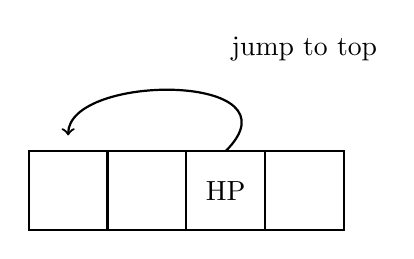
\begin{tikzpicture}
                % Draw the rectangles representing the queue
                \draw[thick] (0,0) rectangle (1,1);
                \draw[thick] (1,0) rectangle (2,1);
                \draw[thick] (2,0) rectangle (3,1);
                \draw[thick] (3,0) rectangle (4,1);
                
                % Arrows to represent "jump to top"
                \draw[->, thick] (2.5, 1) .. controls (3.5, 2) and (0.5, 2) .. (0.5, 1.2);
                
                % Label for high priority
                \node at (2.5, 0.5) {HP};
                
                % Label for "jump to top"
                \node at (3.5, 2.3) {jump to top};
            \end{tikzpicture}
        \end{center}
    \end{definition}